\section{eo\-Pop\-Stat$<$ EOT $>$ Class Template Reference}
\label{classeo_pop_stat}\index{eoPopStat@{eoPopStat}}
Thanks to MS/VC++, {\bf eo\-Param}{\rm (p.\,\pageref{classeo_param})} mechanism is unable to handle std::vectors of stats.  


{\tt \#include $<$eo\-Pop\-Stat.h$>$}

Inheritance diagram for eo\-Pop\-Stat$<$ EOT $>$::\begin{figure}[H]
\begin{center}
\leavevmode
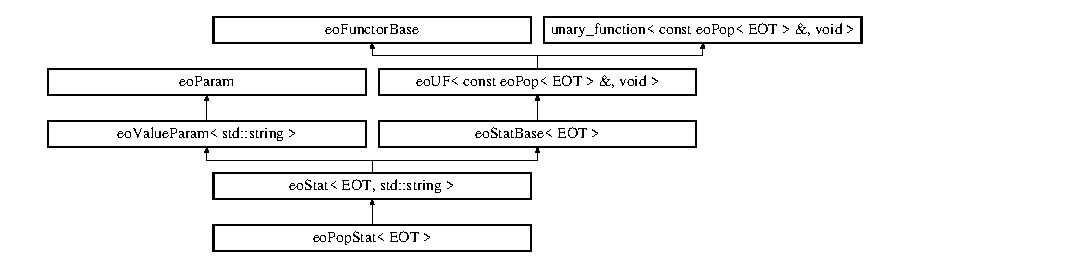
\includegraphics[height=3.15315cm]{classeo_pop_stat}
\end{center}
\end{figure}
\subsection*{Public Member Functions}
\begin{CompactItemize}
\item 
{\bf eo\-Pop\-Stat} (unsigned \_\-how\-Many=0, std::string \_\-desc=\char`\"{}\char`\"{})
\begin{CompactList}\small\item\em default Ctor, void std::string by default, as it appears on the description line once at beginning of evolution. \item\end{CompactList}\item 
void {\bf operator()} (const {\bf eo\-Pop}$<$ {\bf EOT} $>$ \&\_\-pop)
\begin{CompactList}\small\item\em Fills the {\bf value()}{\rm (p.\,\pageref{classeo_value_param_a2})} of the {\bf eo\-Param}{\rm (p.\,\pageref{classeo_param})} with the dump of the population. \item\end{CompactList}\end{CompactItemize}
\subsection*{Private Attributes}
\begin{CompactItemize}
\item 
unsigned {\bf combien}\label{classeo_pop_stat_r0}

\end{CompactItemize}


\subsection{Detailed Description}
\subsubsection*{template$<$class EOT$>$ class eo\-Pop\-Stat$<$ EOT $>$}

Thanks to MS/VC++, {\bf eo\-Param}{\rm (p.\,\pageref{classeo_param})} mechanism is unable to handle std::vectors of stats. 

This snippet is a workaround: This class will \char`\"{}print\char`\"{} a whole population into a std::string - that you can later send to any stream This is the plain version - see eo\-Pop\-String for the Sorted version

Note: this Stat should probably be used only within eo\-Std\-Out\-Monitor, and not inside an {\bf eo\-File\-Monitor}{\rm (p.\,\pageref{classeo_file_monitor})}, as the {\bf eo\-State}{\rm (p.\,\pageref{classeo_state})} construct will work much better there. 



Definition at line 51 of file eo\-Pop\-Stat.h.

\subsection{Constructor \& Destructor Documentation}
\index{eoPopStat@{eo\-Pop\-Stat}!eoPopStat@{eoPopStat}}
\index{eoPopStat@{eoPopStat}!eoPopStat@{eo\-Pop\-Stat}}
\subsubsection{\setlength{\rightskip}{0pt plus 5cm}template$<$class EOT$>$ {\bf eo\-Pop\-Stat}$<$ {\bf EOT} $>$::{\bf eo\-Pop\-Stat} (unsigned {\em \_\-how\-Many} = {\tt 0}, std::string {\em \_\-desc} = {\tt \char`\"{}\char`\"{}})\hspace{0.3cm}{\tt  [inline]}}\label{classeo_pop_stat_a0}


default Ctor, void std::string by default, as it appears on the description line once at beginning of evolution. 

and is meaningless there. \_\-how\-Many defaults to 0, that is, the whole population 

Definition at line 61 of file eo\-Pop\-Stat.h.

\subsection{Member Function Documentation}
\index{eoPopStat@{eo\-Pop\-Stat}!operator()@{operator()}}
\index{operator()@{operator()}!eoPopStat@{eo\-Pop\-Stat}}
\subsubsection{\setlength{\rightskip}{0pt plus 5cm}template$<$class EOT$>$ void {\bf eo\-Pop\-Stat}$<$ {\bf EOT} $>$::operator() (const {\bf eo\-Pop}$<$ {\bf EOT} $>$ \& {\em \_\-pop})\hspace{0.3cm}{\tt  [inline, virtual]}}\label{classeo_pop_stat_a1}


Fills the {\bf value()}{\rm (p.\,\pageref{classeo_value_param_a2})} of the {\bf eo\-Param}{\rm (p.\,\pageref{classeo_param})} with the dump of the population. 

Adds a \par
 before so it does not get mixed up with the rest of the stats that are written by the monitor it is probably used from. 

Implements {\bf eo\-UF$<$ const eo\-Pop$<$ EOT $>$ \&, void $>$} {\rm (p.\,\pageref{classeo_u_f_a1})}.

Definition at line 68 of file eo\-Pop\-Stat.h.

References eo\-Value\-Param$<$ std::string $>$::value().

The documentation for this class was generated from the following file:\begin{CompactItemize}
\item 
eo\-Pop\-Stat.h\end{CompactItemize}
